% !TeX encoding = UTF-8
% !TeX spellcheck = de_DE
% !TeX root = ./mainDoc.tex

\section{Delegation und Mixins}

Ein Mechanismus zum Code-Reuse in klassischen Sprachen ist die Vererbung. Dazu wird eine Hierarchie aufeinander aufbauender Klassendefinitionen definiert. Die tiefer liegende Subklassen \emph{erben} alle Eigenschaften der darüber liegender Superklassen und können sie verwenden. Die tiefer liegenden Subklassen können eigene Eigenschaften ergänzen und Eigenschaften der darüber liegenden Superklassen verändern. Man spricht davon, dass Methoden oder Properties überschrieben werden. Man kann sich das vorstellen, wie Baupläne auf transparentem Papier, die übereinandergelegt werden. 

Wenn eine Instanz einer Subklasse erzeugt wird, so entsteht ein neues Objekt nach der Definition, die sich aus der Summe der Klassendefinitionen der Klassenhierarchie ergibt. Das neue Objekt ist eine materialisierte Kopie dieser Summendefinition.

\subsection{Prototypische Vererbung und Delegation}

Da JavaScript nicht auf Klassen basiert, sondern auf Objekten, die zueinander in Beziehung stehen, ist dieser Mechanismus in der Form nicht verfügbar. Javascript bietet anstelle dessen den \emph{Delegation}-Mechanismus entlang der Prototype-Chain.

%, der häufig auch als Vererbung bezeichnet wird und darauf beruht, dass jedes Objekt in Javascript einen Link zu einem weiteren Objekt hat, der als [[Prototype]]-Link bezeichnet wird. 
%Einen solchen [[Prototype]]-Link besitzt jedes Objekt in Javascript. Dieser Link referenziert entweder ein weiteres Objekt, oder aber den primitiven \texttt{null}-Wert. Die Abfolge dieser Links wird als \emph{Prototype-Chain} bezeichnet und geht vom aktuellen Objekt so lange weiter, bis \texttt{null} erreicht wird. In der Regel ist das letzte in der Prototype-Chain referenzierte Objekt das in JavaScript eingebaute Objekt \texttt{Object.prototype}, dessen [[Prototype]] auf \texttt{null} zeigt.
%
%Mit Hilfe dieses Mechanismus kann man in JavaScript Objektgeflechte aufbauen, die sich ähnlich verhalten wie Klassenhierarchien mit Vererbung in klassischen OO-Sprachen. Technisch gesehen handelt es sich aber nicht um Klassenintantiierungen mit geerbten Eigenschaften, sondern um einen Delegationsmechanismus zwischen Objekten. In \citep[p. 116]{SimpsonThisobjectprototypes2014} wird dies als "`OLOO (objects linked to other objects)"'-Stil bezeichnet.
%
%Um zu verstehen, wie die Prototype-Delegation in JavaScript funktioniert muss man zunächst verstehen, wie der Zugriff auf eine Property eines Objekts abläuft.
%Ein Objekt in JavaScript ist wie ein \texttt{\{key: value\}}-Store organisiert, in dem zu jedem Property-Namen (\texttt{key}) der entsprechende primitive Wert oder eine Referenz auf ein weiteres Objekt (\texttt{value}) gespeichert ist.
%Wenn eine Property oder Methode auf einem Objekt aufgerufen wird, so wird zunächst im Objekt selber geschaut, ob es eine passende Property diesen Namens gibt gibt. Ist das der Fall, so wird der zugehörige Wert zurückgegeben. Wird aber keine passende Property gefunden wird, so folgt JS dem [[Prototype]]-Link des Objekts und schaut in dem dadurch referenzierten Objekt nach der gesuchten Property. So wird die gesamte Prototype-Chain abgesucht, bis sie entweder zu Ende ist, oder die gesuchte Property gefunden wurde. Die Suche wird abgebrochen, sobald eine Property passenden Namens gefunden wurde. Dadurch können Properties am Anfang der Prototype-Chain die Properties von Objekten weiter am Ende der Kette überdecken (\emph{shadowing}). Diese verdeckten Properties können dann nur noch über die direkte Angabe des enthaltenden Objekts zugegriffen werden. 
%
%Während der Traversierung der Prototype-Chain bleibt der \texttt{this}-Zeiger immer an das Ursprungsobjekt am Anfang der Kette gebunden. Das bedeutet, dass auch Funktionen, die am ende der Kette stehen trotzdem auf dem Ursprungsobjekt am Anfang der Kette operieren.



%- Auch JS bietet einen Mechanismus, der als Vererbung bezeichnet wird
%- Dieser läuft über die sogenannte Prototype-Chain
%- Es handelt sich eher um Delegation als um Vererbung
%	- Wenn eine Property oder Methode auf einem Objekt aufgerufen wird, so wird zunächst im Objekt selber geschaut, ob es eine passende Property gibt
%	- Wenn keine passende Property gefunden wird, dann folgt JS dem [[Prototype]] Link und schaut in dem dadurch referenzierten Objekt nach der gesuchten Property
%	- Es wird die gesamte \emph{Prototype-Chain} abgesucht, bis diese entweder zu Ende ist, oder eine passende Property gefunden wurde.
%	- Es wird abgebrochen, sobald eine passende Property gefunden wird.
%	- Wenn es sich um eine Funktion handelt, so ist \texttt{this} immer noch an das Ursprungsobjekt am Anfang der Prototype-Chain gebunden

%\subsection{Prototypische Vererbung über Delegation}

Der [[Prototype]]-Link eines jeden Objekts ist zugreifbar und kann sowohl gelesen als auch gesetzt werden. Der Prototyp ist über die Funktionen \texttt{Object.get\-Proto\-typeOf(obj)} und \texttt{Object.setProto\-typeOf(obj, proto)}, und seit ES6 auch über die eigenen Property \texttt{.\_\_proto\_\_} zugreifbar. Bei Objekten, die über einen Konstruktoraufruf erzeugt werden, wird der [[Prototype]]-Link bei der Erzeugung auf das über die Property \texttt{.prototype} der Konstruktorfunktion referenzierte Objekt gesetzt.

Mit Hilfe der Prototype-Chain und der Möglichkeit, den Prototypen eines Objekts zu manipulieren, lässt sich klassenähnliches Verhalten in JavaScript simulieren: (Wert"~) Pro\-per\-ties werden in der Konstruktorfunktion auf dem neu erstellten Objekt definiert. Sie sind für jedes später über den Konstruktor erzeugte  Objekt genau einmal vorhanden. Methoden (Verhaltens-Properties) werden auf dem Prototypen des Objekts definiert, auf den \texttt{.prototype} der Konstruktorfunktion zeigt. Sie sind lediglich einmal auf dem [[Prototype]]-Objekt vorhanden, auf das alle über den Konstruktor erzeugten Objekte verlinkt sind. Auch auf dem Prototypen können Wert-Properties definiert werden, das funktioniert aber häufig nicht so, wie gewünscht.

Ein Beispiel eines Zählerobjekts ist in Listing \ref{codesnips/protoCounterConstructor.js} zu sehen:

\insertcode{codesnips/protoCounterConstructor.js}{Erzeugung eine \texttt{Counter}-"`Klasse"' und Instantiierung zweier \texttt{Counter}-Objekte.}

Zunächst wird eine Konstruktorfunktion definiert, auf deren \texttt{.prototype}-Objekt die für einen Zähler notwendigen Properties und Funktionen definiert sind.
Sodann werden über Konstruktoraufrufe zwei Zählerobjekte erzeugt. Die Zähler werden mehrfach inkrementiert und das Ergebnis abgefragt. Es ergibt sich folgende (überaschende) Ausgabe:
\begin{verbatim}
one.counter? false
one.counter? true
two.counter = 0;	two.counterObj.value = 3;
one.counter = 3;	one.counterObj.value = 4;
two.counter = 1;	two.counterObj.value = 4;
\end{verbatim}

Diese Ausgabe lässt sich wie folgt erklären: Die Wert-Properties \texttt{counter} und \texttt{coun\-ter\-Obj} sind auf dem Prototypen \texttt{Counter.prototype} definiert. Das durch den Konstruktoraufruf \texttt{new Counter('one');} erzeugte Objekt hat keine eigene Property mit dem Namen \texttt{counter}. Sobald jedoch die Funktion \texttt{inc()} aufgerufen wird, wird eine solche Property direkt auf dem Objekt \texttt{one}, auf das die \texttt{this}-Referenz beim Funktionsaufruf zeigt, angelegt und mit einem Wert belegt. Das liegt daran, das bei schreibenden Zugriffen auf eine Property nicht erst ein passendes Objekt entlang der Prototype-Chain gesucht wird, sondern direkt eine eigene Property angelegt wird, wenn der Schreibzugriff auf eine noch nicht existierende Property des Objekts erfolgt. 

Die Zeile \texttt{this.counter++;} wird ausgeführt als \texttt{one.counter = one.counter + 1}. Es wird die Property \texttt{counter} auf dem Objekt \texttt{one} gesucht und auf \texttt{one.\_\_proto\_\_} gefunden. Dazu wird 1 addiert und es wird der Property \texttt{one.counter} zugewiesen. Da diese Property auf \texttt{one} noch nicht existiert, wird sie angelegt. Ab nun hat \texttt{one} eine eigene Property \texttt{counter}, welche \texttt{one.\_\_proto\_\_.counter} verdeckt.

Die Zeile \texttt{this.counterObj.value} dagegen wird als \texttt{one.counterObj.value = one.} \texttt{counterObj.value + 1} ausgeführt. Hier wird bei beiden Zugriffen auf \texttt{one.counterObj} nur lesend zugegriffen. Der Schreibzugriff erfolgt auf die darin enthaltene \texttt{value}  Property.
In beiden Fällen wird für \texttt{one.counterObj} die Objektreferenz auf \texttt{one.\_\_proto\_\_} gefunden. Die in diesem referenzierten Objekt enthaltene Property \texttt{value} wird ausgelesen, inkrementiert und gespeichert. Die Objektreferenz \texttt{one.counterObj} bleibt dabei unverändert. Sie ist für beide Objekte \texttt{one} und \texttt{two} lediglich einmal auf dem durch \texttt{Counter.prototype} referenzierten Objekt vorhanden.
Die Abbildung \ref{shadowing} veranschaulicht die Situation.
\begin{figure}[!h]
	\centering
	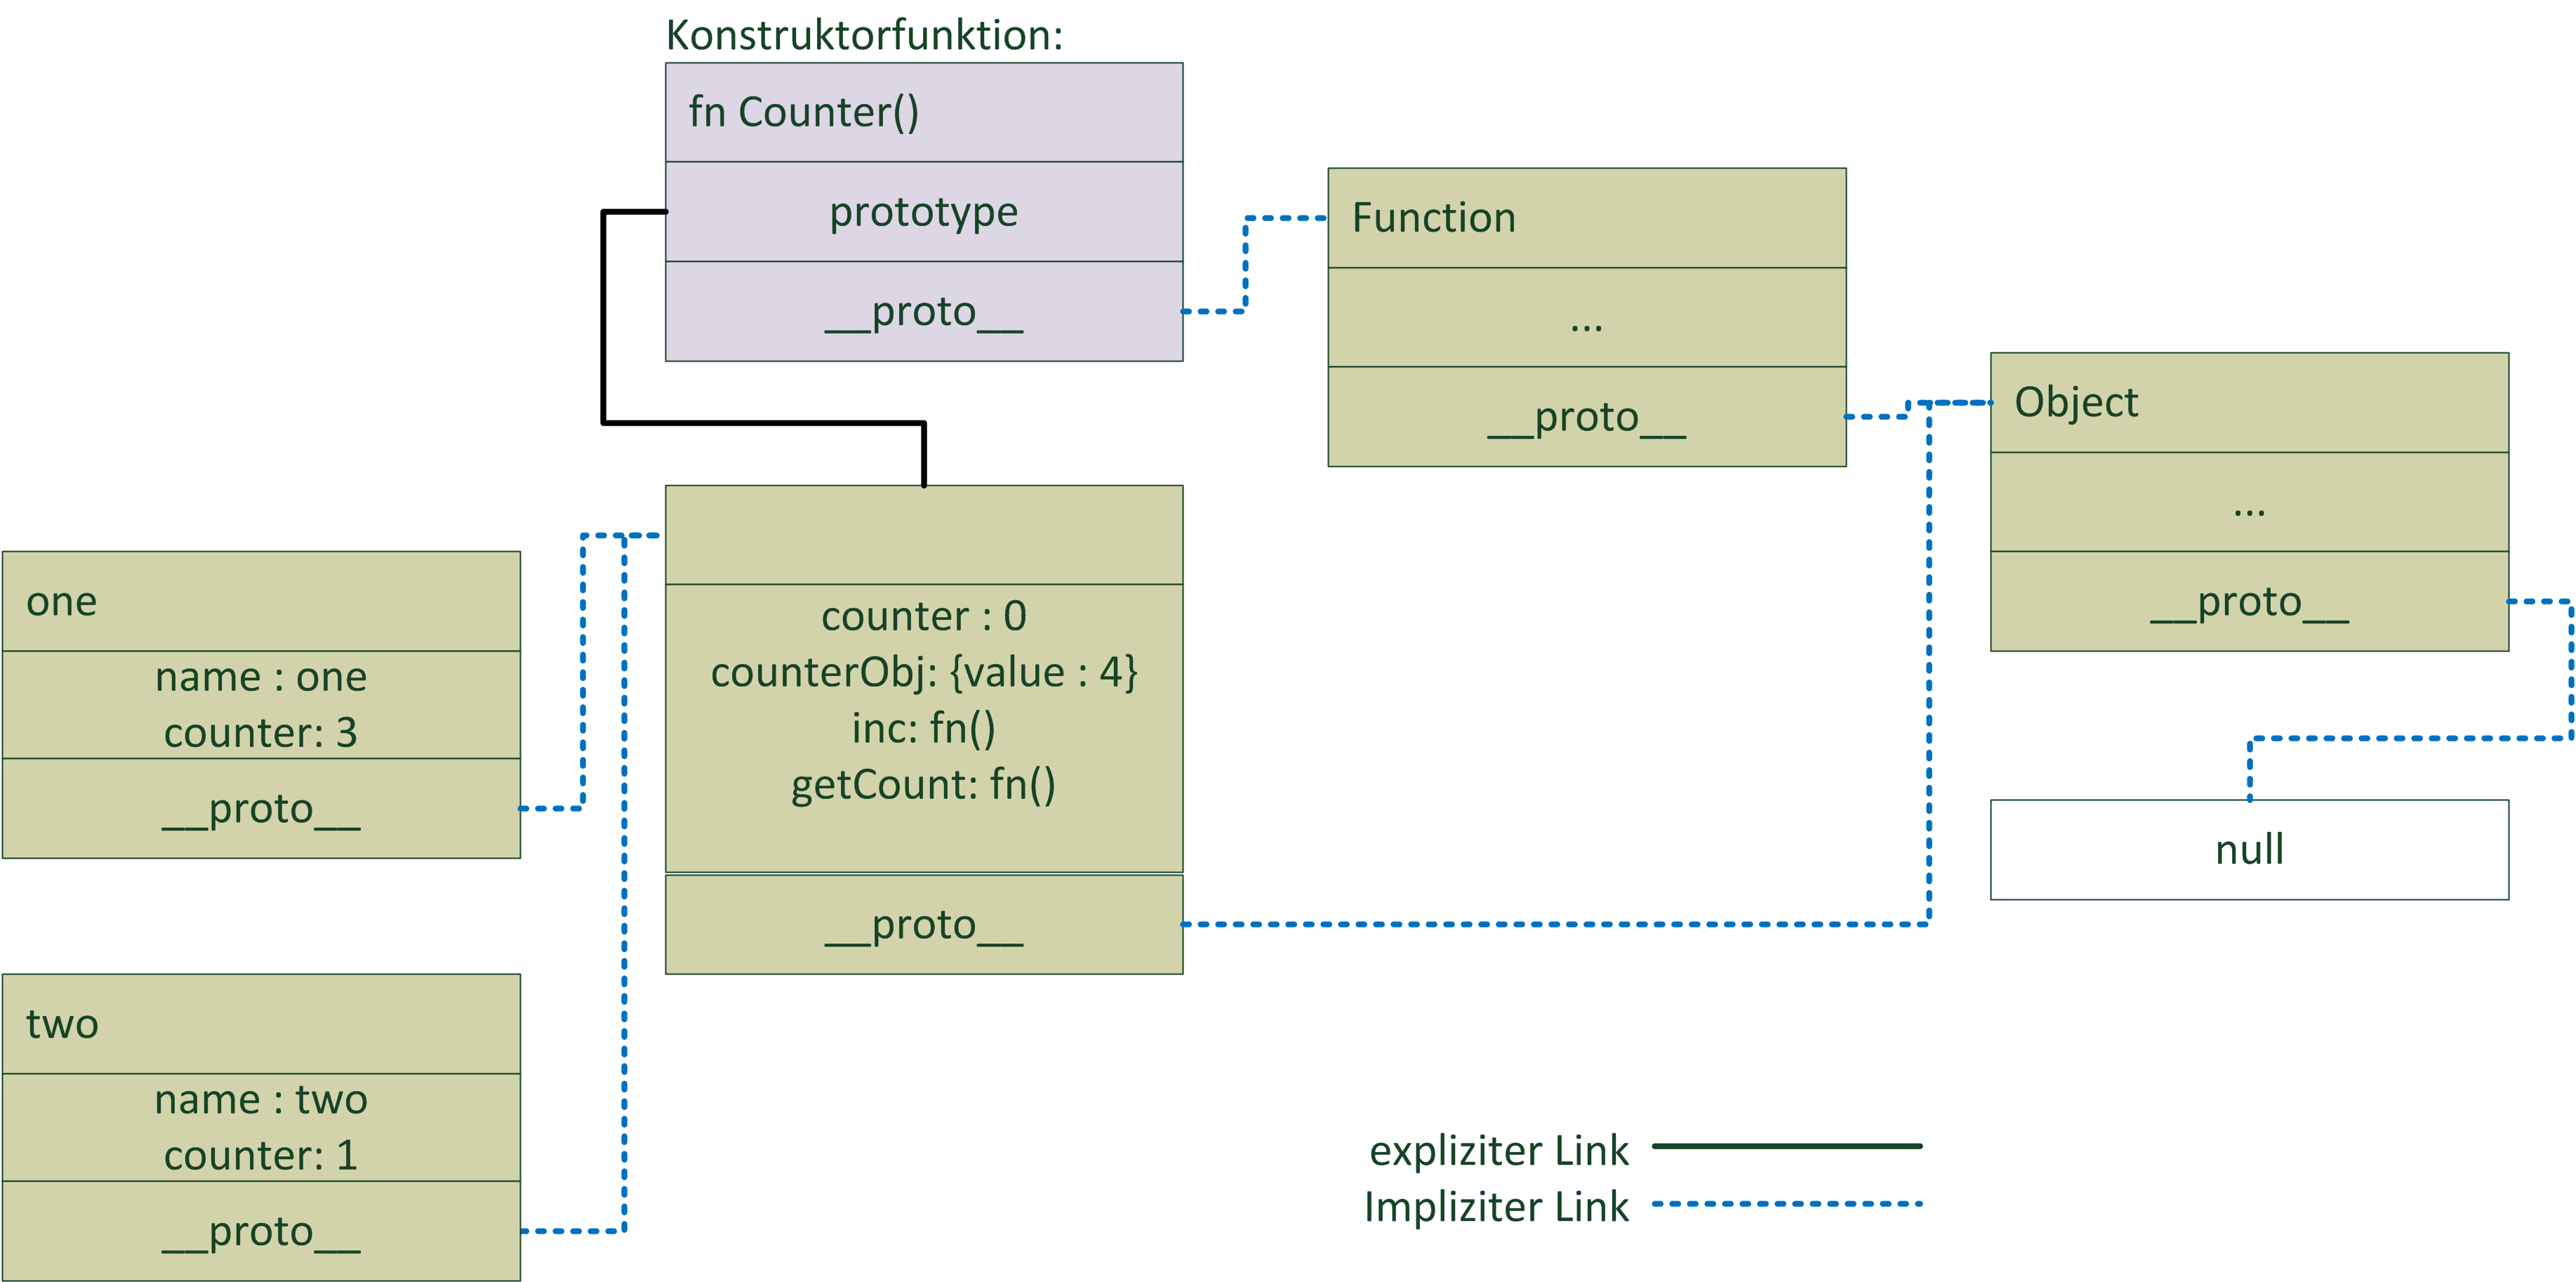
\includegraphics[width=\textwidth]{images/CounterPrototypeChain.png}
	\caption{\label{shadowing}Objektgeflecht des Zählerbeispiels.}
\end{figure}

%In diesem Beispiel wird deutlich, dass die beiden Objekte \texttt{one} und \texttt{two} \emph{nicht} wie in der klassischen Objektorientierung eine materialisierte Kopie der Klassendefinition von \texttt{Counter} sind, die alle Eigenschaften und Properties von \texttt{Counter.prototype} erben, sondern in JavaScript lediglich Objekte exisitieren, die mit anderen Objekten verlinkt sind und über diese Links Aufgaben delegieren. Beim Aufbau von vererbungsähnlichen Delegationshierarchien muss die Programmiererin immer im Auge behalten, auf welchem Objekt eine Property gerade definiert ist und ob es sich um einen primitiven Wert oder eine Referenz handelt.\footnote{Mit der Einführung des Klassenmechanismus über \texttt{class} sind viele Automatismen eingeführt wurden, welche der Programmiererin den Eindruck einer klassischen OO-Sprache vermitteln. Doch auch ES6-Klassen werden unter der Haube auf den dargestellten Delegationsmechanismus abgebildet.}

\skippingparagraph

Ausgehend von dem gezeigt Beispiel lassen sich natürlich auch in JavaScript mehrstufige Delegations-Hierarchien erstellen, die einer Vererbungshierarchie in klassischen OO-Sprachen ähnelt. Zur Verdeutlichung des Prinzips sei ein kurzes Beispiel gezeigt. Es sollen, wie in Abbildung \ref{protoInheritance} dargestellt, vier Objekte erstellt werden.

\begin{figure}[!h]
	\centering
	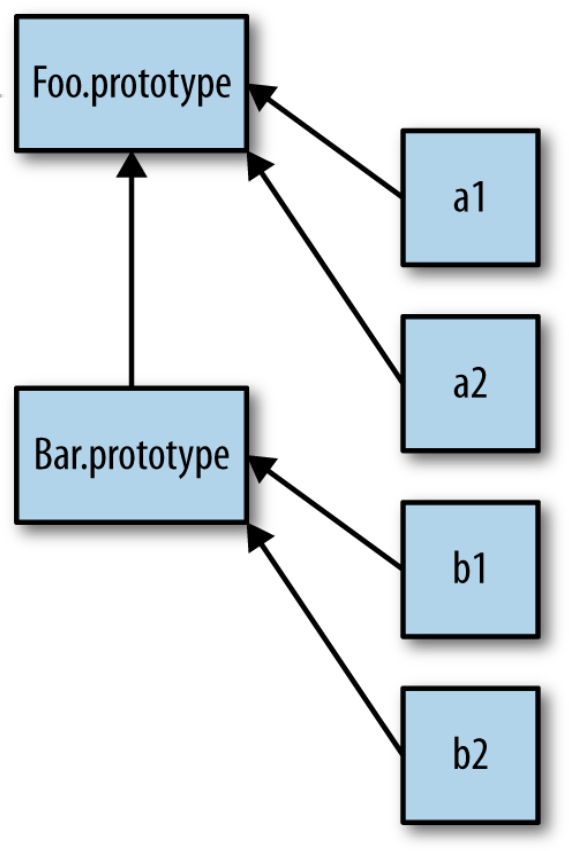
\includegraphics[width=0.3\textwidth]{images/prototypalInheritance.png}
	\caption{\label{protoInheritance}Prototypische Vererbung / Delegationshierarchie (aus \citep[p. 93]{SimpsonThisobjectprototypes2014})}
\end{figure}

Dies lässt sich wie im Listing \ref{codesnips/protoInheritanceSimpson.js} gezeigt programmieren. Zunächst wird eine Konstruktorfunktion für \texttt{Foo} erstellt, auf deren \texttt{.prototpye}-Objekt eine Funktion \texttt{identify} definiert wird. Dieser Prototyp wird als zu verlinkendes Delegate-Objekt an die zweite Konstruktorfunktion \texttt{Bar} über deren \texttt{.prototype}-Link angebunden. Im \texttt{Bar}-Konstruk\-tor wird explizit \texttt{Foo.call(this)} aufgerufen. Es handelt sich dabei um Method-Borrow\-ing, so dass \texttt{Foo} ein explizites \texttt{this}-Binding auf das Objekt erhält, das beim Konstruktoraufruf von \texttt{Bar} neu erzeugt wurde und auf diesem Objekt Properties setzen kann. 

Auch auf dem \texttt{Bar.prototype}-Objekt ist eine Funktion \texttt{identify} definiert. Diese "`überschreibt"' die gleichnamige Funktion auf \texttt{Foo.prototype}, da sie in der Prototype-Chain früher gefunden wird. Es ist zu erkennen, dass der in klassichen Sprachen übliche Aufruf der überschriebenen Funktion deutlich umständlicher ist als der klassisch übliche Aufruf \texttt{super()}. In JavaScript ist man daher bemüht das Überschreiben zu vermeiden, wenn die überschriebene Property noch benötigt wird.


\insertcode{codesnips/protoInheritanceSimpson.js}{Erzeugung einer mehrstufigen prototypischen Vererbungs-/Delegations-Hierarchie (frei nach \citep{SimpsonThisobjectprototypes2014}, p. 101)}


\subsection{Vererbung durch Kopieren}

Im vorangehenden Abschnitt wurde gezeigt, wie die in JavaScript enthaltene Delegation zwischen OLOO (Objects Linked to Other Objects) funktioniert, und wie man mit ihrer Hilfe einen Mechanismus aufsetzen kann, der der klassischen Vererbung sehr nahe kommt. Es wurde dabei im \texttt{Counter}-Beispiel auch aufgezeigt, dass bei der Objektinstantiierung keine Kopien von Klassendefinitionen erstellt werden, sondern lediglich Objekte, die über Ihre Prototype-Chain auf andere, bereits bestehende Objekte verlinkt sind. Dies kann zu unerwartetem Verhalten führen, wenn nicht genau darauf geachtet wird, ob eine Property einen primitiven Wert enthält oder auf ein Objekt refrenziert.

In den vorangehenden Beispielen wurde auch deutlich, dass --im Gegensatz zu klassischen Sprachen-- Objekte in JavaScript dynamisch sind und jederzeit auch nach Erstellung verändert werden können. So wurden den \texttt{.prototype}-Objekten nach ihrer Erstellung Funktions-Properties hinzugefügt.

Die Möglichkeit, Objekte nach ihrer Erstellung zu verändern, lässt sich nutzen, um Code-Wiederverwendung nicht über Delegation zu erreichen, sondern über automatisierte Kopien von Properties. Es lässt sich einfach eine Hilfsfunktion \texttt{extend} schreiben, die ein bestehendes Objekt mit den Properties eines anderen Objekts erweitert. Die Vererbung findet hier durch Kopieren statt.

In Listing \ref{codesnips/extendStefanov.js} wird ein \texttt{kid} Objekt dadurch erzeugt, dass in ein leeres Objekt alle eigenen Properties des \texttt{dad}-Objekts einkopiert werden. Wichtig zu sehen ist dabei, dass diese beiden Objekte \texttt{nicht} über die Prototype-Chain verbunden sind. Es werden lediglich die im Elternobjekt vorhandenen eigenen Properties kopiert. Es wird eine sogenannte \emph{flache} Kopie (\emph{shallow copy}) des Elternobjekts im Kind-Objekt erzeugt. Die gezeigte Funktion \texttt{extend} ist seit ES6 auch im JavaScript Sprachstandard enthalten und es kann einfacher \texttt{Object.assign(target, \ldots sources)} geschrieben werden.

\insertcode{codesnips/extendStefanov.js}{"`Vererbung"' durch Kopieren (frei nach \citep{StefanovJavaScriptpatternsbuild2010}, p. 133f.)}

Auch hier besteht das Problem wie im \texttt{Counter}-Beispiel, dass Properties, die Referenzen auf andere Objekte sind, von beiden Kopien aus auf das gleiche Ursprungsobjekt zeigen und damit keine eigenständigen, gedoppelten Werte enthalten. 
Das ist in der Regel nicht gewünscht, und es müssen entsprechende Setter-Funktionen programmiert werden, die den Inhalt solcher Referenzen durch eigene Objekte ersetzen, und nicht nur den Wert einzelner Objektproperties verändern. In diesem Beispiel sollte die Funktion \texttt{Array.concat()} anstelle von \texttt{Array.push()} verwendet werden. \texttt{Array.concat()} gibt immer ein neues Array zurück, während \texttt{Array.push()} das ursprüngliche Array verändert.

Eine (selten genutzte) Alternative besteht darin, eine sogenannte \emph{tiefe} Kopie (\emph{deep copy}) zu erstellen, die Objekt- und Array-Referenzen rekursiv auflöst, und entsprechend neue Werte im Empfängerobjekt erstellt. Eine solche tiefe Kopierfunktion ist in Listing \ref{codesnips/extendDeepStefanov.js} zu sehen.

\insertcode{codesnips/extendDeepStefanov.js}{"`Vererbung"' durch \emph{tiefes }Kopieren (frei nach \citep{StefanovJavaScriptpatternsbuild2010}, p. 134)}

Mit Hilfe der \texttt{extendDeep} Funktion wird das \texttt{parent}-Objekt im \texttt{child}-Objekt vollständig dupliziert. Dadurch können sich die beiden Objekte danach nicht mehr beeinflussen. Eine solche tiefe Kopie ist jedoch eine sehr teure Operation und meist nicht notwendig. Der Einsatz einer tiefen Kopierfunktion für die Wiederverwendung von Code ist nur in Ausnahemefällen sinnvoll, die im Vorfeld genau analysiert werden müssen. In den meisten Fällen ist die sorgfältige Implementierung geeigneter Setter vorzuziehen, die selektiv Objekte austauschen, wenn darin enthaltene Werte verändert werden sollen.

\subsection{Object-Mixins für den orthogonalen Code-Reuse}
Durch bisher gezeigten Beispiele der Code-Wiederverwendung per Delegation oder per Kopie wurde eine baumartige Hierarchie aufgebaut, wie sie typischerweise in allen Vererbungshierarchien in OO-Sprachen mit Einfachvererbung entsteht. Eine solch strenge Hierarchie, in der jede Entität genau einen Vorgänger hat, von dem Eigenschaften übernommen werden können, ist in der Praxis häufig nicht ausreichend. Es gibt in der Realität in fast allen Bereichen Anwendungsfälle, die sich mit einer solchen Baumstruktur nicht darstellen lassen. %Es gibt Querverbindungen zwischen Modellaspekten, die \emph{orthogonal} zu dieser Baumstruktur stehen.

Als Beispiel sei das Modell einer Firma und ihrer Mitarbeitern genannt: Ein \texttt{Entwick\-ler} ist ein \texttt{Angestellter}, der eine \texttt{Person} ist. Daneben gibt es noch einen \texttt{Produktions\-mitarbeiter}, der ein \texttt{Angestellter} ist, der eine \texttt{Person} ist. Dieses auf den ersten Blick einleuchtende Modell bricht, sobald ein externer \texttt{Entwickler} in der Firma beschäftigt wird, der selber ein \texttt{Freelancer} ist. In diesem Fall  kann die Realität nicht über einen einfachen Baum modelliert werden. Es kommen Eigenschaften hinzu, die zu der ursprünglich verwendeten Taxonomie \emph{orthogonal} sind. 
%In klassischen Sprachen lässt sich solch ein Problem teilweise durch Mehrfachvererbung modellieren. 

Ein Ansatz zur Modellierung solcher orthogonaler Beziehungen, die nicht einer strengen Hierarchie gehorchen, wird als \emph{Mixin} bezeichnet. 

Der Begriff des Mix-In wurde laut Wikipedia\footnote{\url{https://en.wikipedia.org/wiki/Mix-in}} ursprünglich von einem Eis-Verkäufer geprägt, der aus den immer gleichen Grundsorten (Vanille, Schokolade, \ldots) und weiteren Zutaten (Smarties, Schoko-Chips, Gummibärchen, Kekse, \ldots) eine Unmenge an spezialisierten Eiscremesorten anbieten konnte, die individuell nach Kundenwunsch zubereitet wurden. Er benutzte eine Grundsorte als Ausgangsbasis und mixte weitere Zutaten nach Kundenwunsch unter, so dass ein neuer individueller Geschmack entstand. 

Übertragen auf klassische OO-Programmierung, stellen die baumartigen Vererbungshierarchien aus Super- und Subklassen die Grundzutaten dar. Die zusätzlichen Bestandteile werden mit dem dazu orthogonalem Verhalten identifiziert, das je nach Bedarf hinzugefügt werden kann. Das zuzufügende Verhalten kann in der Sprache der klassischen Objektorientierung als Definition einer \emph{abstrakten Subklasse} bezeichnet werden.

\begin{quote}
A mixin is an abstract subclass; i.e. a subclass definition that may be applied to different
superclasses to create a related family of modified classes.  \citep{BrachaMixinbasedInheritance1990}
\end{quote}

Diese abstrakte Subklasse kann für sich gesehen nicht instantiert werden. Sie kann nur auf eine konkrete Basisklasse angewendet werden, und damit ihr Verhalten dem Verhalten der Basisklasse hinzufügen. Die Basisklasse muss dazu bestimmte Garantien bezüglich ihrer Implementierung geben, damit die erweiterte Funktionalität zur Verfügung gestellt werden kann. Die Verwendung von Mixins in klassischen OO-Sprachen bedarf der Unterstützung der Sprache selber, deren Klassendefinitionen und Objektinstantiierung die Idee einer abstrakten Subklasse, die auf eine konkrete Superklasse angewendet wird, implementieren müssen. Die meisten klassischen OO-Sprachen haben ein Modell implementiert, bei der die Konkretisierung von abstrakten Superklassen zu konkreten Subklassen, also von oben nach unten, geht. Dieses Modell lässt sich nicht ohne weiteres umkehren, weswegen Mixins nicht in vielen Sprachen unterstützt werden.\footnote{Eine Liste von Sprachen, die Mixins direkt unterstützen, findet sich z. B. in \url{https://en.wikipedia.org/wiki/Mixin\%23Programming_languages_that_use_mixins}
}


\begin{figure}[h]
	\centering
	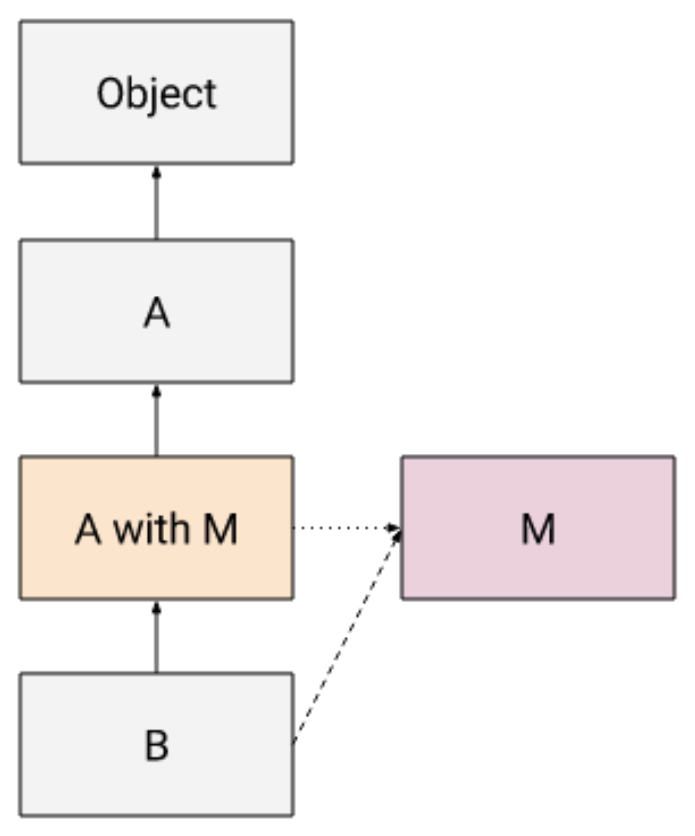
\includegraphics[width=0.3\textwidth]{images/mixinAbstractSubClass.png}
	\caption{\label{mixinAbstractSubClass}Die abstrakte Mixinklasse \texttt{M} angewandt auf die Basisklasse \texttt{A} in der Vererbungshierarchie \texttt{class B extends A with M \{\}}(\citep{FagnaniRealMixinsJavaScript2015})}
\end{figure}

\skippingparagraph

JavaScript hat keine Klassen. Es gibt lediglich Objekte und diese Objekte sind zur Laufzeit dynamisch veränderbar. Damit ergibt sich als direkte Konsequenz aus der im vorigen Abschnitt aufgezeigten einfachen "`Wiederverwendung durch Kopieren"' die Möglichkeit, das Verhalten eines Objekts in ein anderes bestehendes Objekt zu mixen. Der in klassischen Sprachen recht aufwändige Mixin-Mechanismus lässt sich in JavaScript auf eine einfache Kopie zurückführen.

In einer Grundform ist eine flache Kopie der Properties des Mixin-Objekts auf das Empfängerobjekt ausreichend, um eine Mixin-Funktionalität in Javascript zur Verfügung zu stellen. Dieser Vorgang wird auch als "`concatenative sharing"' (\citep{BraithwaiteWhyAreMixins2016}) bezeichnet, da schlicht die Properties des Mixin-Objekts an das zu erweiternde Objekt angehängt werden. In der Vergangenheit wurden dazu meist mehr oder weniger aufwändige \texttt{mixin()}-Funktionen aus Bibliotheken verwendet. Seit ES6 ist jedoch die Funktion \texttt{Object.assign(target, \ldots sources)} standardisiert und kann für diesen Zweck genutzt werden.

Im Listing \ref{codesnips/simpleMixin.js} wird gezeigt, wie leicht sich bestehende Objekte durch einfache Erweiterung mit Mixin-Verhalten ergänzen lassen. Es wird auch deutlich, dass die Mixin-Objekte nicht für sich allein stehen können, da sie im Beispiel auf die \texttt{.name}-Property des Empfängerobjekts zugreifen.

\insertcode{codesnips/simpleMixin.js}{Einfache Object-Mixins durch Definition von Mixin-Objekten und Anwenden von \texttt{Object.assign(target, \ldots sources)}}

Bei der vorgestellten Mixin-Technik werden die Empfängerobjekte lediglich durch eine flache Kopie der Mixin-Objekte erweitert. Es ist daher genau wie im vorangehenden Beispiel darauf zu achten, dass Referenzen auf Objekte innerhalb verschiedener Empfängerobjekte zunächst auf das gleiche Objekt zeigen. Während dieses Verhalten bei den Referenzen auf Funktionen (und damit auf Verhalten des Mixins) wünschenswert ist, um Speicher zu sparen, ist bei objektwertigen Properties Vorsicht geboten. Nach der Erweiterung der beiden Objekte \texttt{felix} und \texttt{john} mit dem \texttt{mixDeveloper} gilt \texttt{john.languages === felix.languages}. 
Das bedeutet, dass die \texttt{.languages}-Property beider Objekte auf dasselbe Array-Objekt referenziert (l.~72). 

Im gezeigten Code-Beispiel wurde dafür Sorge getragen, dass dieses Verhalten keine unerwünschten Nebeneffekte hat. Die \texttt{languages} und \texttt{patterns} Arrays werden bei Veränderung ersetzt und nicht modifiziert. Sowohl die Funktion \texttt{initDeveloper} als auch die Funktionen \texttt{addLanguage} bzw. \texttt{addPattern} ersetzen die Arrays und modifizieren damit die Referenzen der Objekte und nicht nur die Werte innerhalb referenzierter Objekte. 

Aufgrund der Verwendung dynamischer Objekte, deren Verhalten und Struktur zur Laufzeit modifiziert werden kann, ist das Mixin-Pattern in JavaScript sehr einfach anzuwenden. Es bedarf keiner zusätzlichen Sprachunterstützung, sondern lässt sich mit den vorhandenen Mitteln einfach erledigen. Das Muster lässt sich auch in Kombination mit der [[Prototype]]-Delegation einsetzen, so dass nicht nur einzelne Objekte wie im Beispiel mit erweiterter Funktionalität ausgestattet werden können, sondern auch deren [[Prototype]]-Delegates. Dies lässt sich in Factory-Funktionen gewinnbringend einsetzen, wenn eine große Menge erweiterter Objekte erzeugt werden soll. 

\skippingparagraph
Trotz des einfachen Einsatzes von Mixins soll nicht verschwiegen werden, dass in der Praxis in größeren Projekten noch einige Details behandelt werden müssen, die den Einsatz etwas komplizierter als im Beispiel gezeigt machen. Dies betrifft insbesondere den Umgang mit namensgleichen Properties. In der gezeigten Methodik "`gewinnt"' das zuletzt eingemixte Objekt und dessen Implementierung einer Property oder eines Verhaltens bestimmt das Verhalten des erweiterten Objekts. Ohne spezielle Vorkehrungen gibt es keine Möglichkeit, die Methoden oder Properties der Vorgängerobjekte zu erreichen. Es kann jedoch per Method-Borrowing explizit aus der überschreibenden Mixin-Methode die gleichnamige Methode des Empfängerobjekts aufgerufen werden (siehe dazu "`explicit pseudopolymorphism"' \citep[p.78]{SimpsonThisobjectprototypes2014}). Eine andere Möglichkeit besteht darin eine aufwändigere \texttt{mixin()}-Funktion zu benutzen, die bei Namensgleichheit eine automatische Konfliktlösung bietet. Dies wird z.~B. in \texttt{react-server.js} realisiert. Dort können für bestimmte Properties sogenannte \texttt{specPolicies} wie \texttt{OVERRIDE\_BASE}, \texttt{DEFINE\_ONCE}, \texttt{DEFINE\_MANY} oder \texttt{DEFINE\_MANY\_MERGED} angegeben werden. Diese zusätzlichen Angaben werden beim Kopieren der Properties entsprechend berücksichtigt. Die Details dieser Implementierung\footnote{
Die Funktion \texttt{mixSpecIntoComponent} lohnt eine weitere Betrachtung der Mechanismen: \url{https://github.com/reactjs/react-rails/blob/ec9e1736d4aac87afe4c4e8ba024b49deadc1d3a/lib/assets/react-source/development/react-server.js} ab Zeile 2828} führen an dieser Stelle jedoch viel zu weit. 


